\chapter{Preliminares}
\todo{Contar qué cuenta este capítulo}
\section{Estado del Arte}
\subsection{Introducción}
Cuando navegamos por internet, es posible identificar características que nos permitan reconocer si un determinado usuario ha visitado nuestro sitio. El método más común para detectarlo es mediante el uso de \textit{cookies}. Este dato nos permite establecer una sesión con el visitante de la página y poder guardar así un estado de la conexión. Además, este identificador de sesión nos permite almacenar las configuraciones personalizadas para esa sesión específica. De esta forma controlamos en todo momento el rastro de nuestros usuarios. Ese trozo de información, llamado \textit{HTTP cookie}\cite{rfc6265}, se genera en el servidor y se intercambia al establecer la conexión. Esto es, la \textit{cookie} se almacena también en el navegador del cliente. \par

A pesar de ello, esta técnica no es suficiente. El usuario puede borrar las \textit{cookies} de su navegador web. En este caso el servidor no le podrá recordar, puesto que la sesión previamente establecida no se puede recuperar y habría que establecer una nueva. Por consiguiente, necesitamos otro enfoque distinto para poder identificar a nuestro usuario con una característica menos volátil. \par

Otro de los parámetros que históricamente se ha empleado para identificar a los internautas en la red ha sido la dirección IP pública origen. Se trata de un identificador utilizado en el protocolo de red TCP/IP, concretamente en la capa de red. Nos permite determinar el origen de las comunicaciones, ya que esta dirección es única. Por tanto, sería razonable obtener este atributo para poder identificar al usuario que está navegando en nuestra página. \par

Esto tampoco es tan sencillo. Hoy en día la mayoría de las direcciones IP suelen ser dinámicas y son asignadas por nuestro \textit{ISP} o Proveedor de Servicios de Internet. Esto quiere decir que cada cierto intervalo de tiempo, el \textit{ISP} va a ir asignando una dirección IP pública a nuestra interfaz de red. En consecuencia, tampoco nos va a ser posible utilizarlo como atributo identificativo, pues para un mismo usuario este valor va a ir variando a lo largo del tiempo. \par

Además de la asignación dinámica de direcciones IP, otro problema asociado a considerar la dirección IP como atributo identificativo es la utilización de técnicas de CG-NAT por algunos \textit{ISP}. Como resultado, distintos dispositivos fuera de nuestra red doméstica podrían compartir la misma dirección IP pública, ya que el \textit{ISP} estaría conectando muchos dispositivos de su red como si de una red interna se tratase. De esta forma nosotros no seríamos capaces de identificar nuestro dispositivo objetivo. \par

Por último, también podríamos considerar posibles intrusiones en una red interna. La dirección IP que resolveríamos pertenecería a un tercer usuario víctima que puede no tener nada que ver con el auténtico dispositivo visitante.  \par

Tanto las direcciones IP públicas como el seguimiento a través de \textit{cookies} fueron consideradas las huellas digitales más fiables durante varios años. Sin embargo, existen otros enfoques que nos permiten llegar a mejores conclusiones a partir de otras técnicas. La alternativa más conocida a las expuestas anteriormente es \textit{browser fingerprinting} o huella digital del navegador web. \par

El método de \textit{browser fingerprinting}\cite{fingerprint} consiste en recopilar información del navegador web en función de las características y configuraciones de este. Esta nueva óptica de identificar al usuario a través de las diversas tecnologías incluidas en los navegadores sin \textit{cookies}, o \textit{cookieless}\cite{cookieless} nos permite afinar más y ser más minuciosos en nuestro objetivo de identificar a los usuarios y monitorizar la actividad que estos realizan en una determinada página web. \par 

Para discutir la efectividad del \textit{browser fingerprinting}, recomendamos el estudio de los siguientes \textit{papers}\cite{panop_paper, javascript_paper, effective_paper}. \par 

En las conclusiones encontramos una paradoja: si bien los primeros estudios aseguraban que la efectividad de este método estaba por encima del 80\% de precisión en cuanto a huellas digitales únicas\cite{panop_paper, javascript_paper}, estudios posteriores no han podido reproducir estos mismos resultados, obteniendo solo un 33.6\%\cite{effective_paper}. \par

La explicación a este fenómeno proviene de la relación entre el desarrollo de recursos efectivos de recopilación de huella digital en navegadores web con el desarrollo de las técnicas de mitigación de las mismas. \par 

Cuantas más procedimientos diferentes de \textit{browser fingerprinting} se emplean, más probable es obtener una huella identificativa de las características del navegador web. Hoy en día, el uso de ciertas métodos aislados no resulta del todo identificativo. Entonces no es necesario hallar un atributo único, sino que es suficiente con encontrar una combinación de atributos que resulte única para poder identificar a un usuario. \par

\subsection{Impacto: peligros y casos de uso}

En esta sección analizaremos las implicaciones que tiene el uso de la identificación de la huella digital en navegadores. Expondremos los casos de usos más frecuentes y los peligros que puede suponer el uso de este recurso. Asimismo, comentaremos algunas posibles implicaciones legales. \par

Al tratarse de un sistema tan efectivo, cabe preguntarse si puede ocasionar a su vez algunos peligros. \par

Sin duda, el principal inconveniente que nos viene a la cabeza es el riesgo que supone para la privacidad. Este método se puede realizar de forma transparente al usuario sin que se dé cuenta ni haga falta pedirle ningún tipo de permiso\cite{challenges}. \par 

La parte legal supone también otro desafío. \par

En Europa, existe el Reglamento General de Protección de Datos (GDPR) que restringe la recopilación de datos personales a no ser que se haga de conformidad a las seis formas legítimas para el tratamiento de datos personales. Estas seis formas son las siguientes: \par

\begin{enumerate}
\item Bajo el consentimiento inequívoco del individuo.
\item Por interés vital del individuo.
\item Por interés público.
\item Necesidad contractual.
\item En cumplimiento de obligaciones legales.
\item Por interés legítimo del responsable del tratamiento de datos.
\end{enumerate}

La GDPR evita mencionar tecnologías específicas para poder estar al día del desarrollo tecnológico más allá de las huellas digitales y las \textit{cookies}\cite{gdpr_eff}. \par 

No obstante, en el reglamento de la GDPR aparecen una serie de considerandos no vinculantes que mencionan el hecho de que las \textit{cookies} y otras huellas digitales pueden ser utilizadas para tanto para elaborar perfiles de personas físicas como para identificarlas. Esto se menciona concretamente en el considerando número 30\cite{gdpr}. \par 

Por tanto, en la práctica, con informar al usuario del empleo de este método, sería suficiente para cumplir con la GDPR\cite{blokt}. Sin embargo, aquellas corporaciones sin acuerdos con Europa podrán seguir recopilando los datos de huellas digitales sin tener en cuenta esta ley. \par

Por supuesto, el agente detrás del empleo este procedimiento va a contar con sus propias motivaciones. De todas maneras, los casos de uso principales suelen ser los siguientes: \par

\begin{itemize}
	\item Realizar un perfil específico de clientes para adaptarse a sus necesidades. Una de las formas es rastrear de qué página viene el usuario y establecer si ese usuario ya ha visitado nuestro sitio anteriormente. En este caso no estamos necesariamente interesados en averiguar la identidad del usuario en sí, tan solo en realizar un perfil. Es el sistema más utilizado por los \textit{data brokers}\cite{data_brocker}. Este es el caso de uso fundamental de la mayoría servicios de publicidad de terceros. \par 
	
	\item Entender la actividad del usuario a través de patrones de comportamiento. Analizando cómo es el flujo de interacción del usuario con nuestra página, podemos llegar a conclusiones muy valiosas. La tecnología de JavaScript es la más utilizada en este aspecto, ya que nos permite analizar la atención del usuario sobre la página (saber si la pestaña se encuentra activa, cuál es la posición del ratón, comprobar si nuestras sugerencias son de verdad atractivos e interesantes para el usuario). Se utiliza mucho en tiendas en línea y redes sociales como estrategia de mercadotecnia. \par 
	
	\item Como consecuencia de los dos casos de uso, la huella digital del navegador puede determinar patrones de comportamiento. De esta forma es posible también precisar si la actividad web está siendo llevada a cabo por un \textit{bot}\cite{bot_paper}. \par 
\end{itemize}

\subsection{Técnicas de \textit{fingerprinting}}

Podemos clasificar las distintas técnicas de detección de huellas digitales en navegadores web en dos grupos distintos: \par 

\begin{itemize}
	\item \textit{Fingerprinting} pasivo: Se limita a explorar el contenido de la petición web sin ejecutar código de forma activa en el navegador del cliente. En este grupo incluiremos la recolección de campos de la cabecera HTTP. En el capítulo~\ref{ch:fuentes_info} explicaremos detalladamente cada uno de los elementos que conforman dicha cabecera. \par 
	
	\item \textit{Fingerprinting} activo:  Se realiza ejecutando código, normalmente JavaScript en el navegador web del cliente que está realizando la petición web. Entre todas las opciones posibles, el sistema operativo, la configuración del idioma, la resolución de pantalla, la detección de \textit{plugins} y el lienzo suelen ser los atributos elegidos para realizar el método activo de identificación de huella digital. En el capítulo~\ref{ch:fuentes_info} se explicará detalladamente cada uno de los elementos JavaScript que hemos obtenido para poder perfilar los navegadores web en nuestro proyecto. \par 
	
\end{itemize}

También podríamos clasificar los distintos sistemas de \textit{browser fingerprinting} teniendo en cuenta el tipo de información a obtener. \par 

Por una parte, podríamos obtener información del \textit{hardware} de la máquina directamente a través de la API de JavaScript. Algunos de estos atributos son: la memoria RAM, el tipo de procesador de la máquina, el nombre de la tarjeta gráfica, el número de núcleos de la CPU o el estado de la batería. \par

Por otra parte, podemos obtener información del sistema operativo, configuraciones del navegados o fuentes y \textit{códecs} de audio y vídeo instalados, entre otros. Todos estos elementos se obtienen del \textit{software} del sistema del cliente. \par 

Entre todo este conjunto de técnicas, las más usadas son: \par 

\begin{itemize}
	\item Recopilar el \textit{User-Agent} del dispositivo: Esto se puede realizar tanto de forma activa como de forma pasiva. En general, en este atributo se anuncia el nombre del navegador web que se está utilizando. Una vez lo conozcamos, sabemos las tecnologías soportadas y podemos profundizar más en nuestra detección de la huella digital. \par 
	
	\item Obtener el lienzo o \textit{Canvas}: La propiedad que tiene el lienzo es que una misma imagen o un mismo texto puede representarse de forma diferente en distintos clientes. Esto depende del número de píxeles del dispositivo, del motor del navegador web, de los formatos de compresión, del sistema operativo y de la unidad de procesamiento gráfico (GPU) que se utilice, principalmente. Se considera esta técnica como una de las más efectivas\cite{never_forget_paper}. Si bien no garantiza la determinar a un usuario, combinado con otros campos casi puede garantizar la identificación inequívoca del mismo. \par 
	
\end{itemize}

Por último, queremos mencionar cuales son los últimos métodos de detección de huella digital en los navegadores que han llamado la atención tanto en estudios académicos como para la industria. Las ideas más disruptivas son: \par

\begin{itemize}
	\item WebGL API: Es una API de JavaScript diseñada para renderizar gráficos 3D. Además, los componentes de WebGL pueden combinarse con otros elementos HTML, como el lienzo\cite{canvas_paper}. Al igual que ocurre con el lienzo, la granularidad de la huella digital dependerá estrechamente del \textit{hardware} del dispositivo, concretamente con la GPU. \par 
	
	\item Web Audio API\cite{audio_w3c}: Esta API está pensada para dar soporte a aplicaciones más avanzadas capaces de sintetizar audio, como controladores de sonido MIDI, y para mejorar la experiencia de usuario al jugar a videojuegos web. La idea que hay detrás obtener una huella digital a través de este sistema es que las señales de audio son procesadas de formas distintas en cada navegador del cliente según el \textit{hardware} y \textit{software} del que disponga. Por eso, en una determinada máquina, los parámetros serán siempre los mismos. \par 
	
	\item Utilización de los niveles de batería: HTML5 implementa la API \textit{Battery Status} que permite extraer valores de carga y descarga de la batería. Si esto es utilizado por un \textit{script} de terceros, pueden vincular esos niveles de batería con las visitas a determinadas web en un intervalo de tiempo. De esta forma se podría obtener la traza de navegación de un usuario\cite{battery_paper}. \par 
	
\end{itemize}

\subsection{Técnicas de evasión}
``Las opciones actuales de los usuarios para mitigar estas amenazas son limitadas, en parte debido a la dificultad de distinguir las rastreando desde el comportamiento benigno.'' (\textit{The Web Never Forgets: Persistent Tracking Mechanisms in the Wild}: \cite{never_forget_paper}) \par 

La mitigación más sencilla para aumentar la seguridad y privacidad de nuestro navegador es por supuesto eliminar funcionalidades. No obstante, elevar nuestro nivel de protección sin degradar la experiencia del usuario siempre es un desafío. \par 

Como resultado, no existe una solución simple, sino que tan solo se pueden implementar medidas de mitigación\cite{mitigations_w3c}. \par 

\begin{itemize}
	\item Modificar de los ajustes del navegador. Cada navegador cuenta con unas opciones configurables. En la mayoría de ellos podemos habilitar funciones de anti-seguimiento. \par
	
	Es posible acceder a las configuraciones avanzadas de nuestros navegadores y deshabilitar funcionalidades y configuraciones que puedan dar demasiados detalles de nuestra huella digital. En Firefox bastaría con ingresar en el recurso \textit{about:config}. Google Chrome cuenta con otra opción equivalente, \textit{chrome://flags/} \par
	
	Otra opción es utilizar navegadores que ya vengan con configuraciones por defecto para evadir varias técnicas de detección de huella digital, como Tor Browser. \par 
	
	\item Utilizar complementos y extensiones para el navegador que modifiquen el comportamiento del navegador\cite{pixelprivacy}). Existe una gran diversidad de complementos que realizan esta labor. Algunos de los más conocidos son \textit{NoScript} y \textit{uMatrix}.
	Permiten una configuración flexible por lo que es posible bloquear solo el código JavaScript y los elementos de Flash que deseemos, sin tener que prescindir de la funcionalidad completa. Es una solución de compromiso que busca el equilibro entre privacidad y funcionalidad. \par
	
	Además del bloqueo de elementos Flash y JavaScript, existen más complementos que modifican las cabeceras HTTP y que alteran algunas APIs de JavaScript para evitar el \textit{fingerprinting}. De esta forma podemos falsear los datos que se van a recopilar sobre nosotros. Como resultado, tanto los métodos activos como pasivos serían mucho menos eficaces. \par 
	
	
	\item Utilizar máquinas virtuales: Es posible virtualizar distintos sistemas operativos con sus respectivos navegadores. De esta forma mantener por separado nuestros distintos intereses, como puedan ser trabajo, ocio, educación, etc. Y utilizar así cada perfil para un fin específico. Por supuesto, siempre podemos borrar la máquina virtual y crear otra nueva\cite{restoreprivacy}. \par 
	
\end{itemize}

Todas estas medidas de mitigación son tan solo esfuerzos técnicos. Cambios en las tecnologías provocarían que las medidas que hoy son eficaces para evitar la huella digital mañana estén desfasadas y resulten inútiles. Por esta razón, sin una regulación efectiva en el campo del derecho, estos trucos y ajustes están destinados a fracasar a largo plazo.  \par 

\section{Tecnologías empleadas}

Existe un abanico muy amplio de tecnologías\cite{web_mozilla} relacionadas con la navegación web. Para dar una primera visión general, vamos a realizar una clasificación de las distintas tecnologías web que hemos utilizado en las siguientes categorías: \par
\begin{itemize}
	\item Tecnologías básicas:
		\begin{itemize}
			\item HTML.
			\item CSS.
			\item HTTP.
		\end{itemize}
	\item Lenguajes de escritura:
		\begin{itemize}
			\item JavaScript y AJAX.
			\item PHP.
			\item JSON.
			\item Web APIs.
		\end{itemize}
	\item Backend:
		\begin{itemize}
			\item XAMPP.
				\begin{itemize}
					\item Apache.
					\item MariaDB.
					\item PhpMyAdmin.
				\end{itemize}
		\end{itemize}
\end{itemize}

A continuación exponemos una breve explicación sobre en qué consiste cada tecnología utilizada y porqué nos hemos decantado por usarla. \par 

\subsection{Tecnologías básicas}

\subsubsection{HTML}
HTML significa Lenguaje de Marcado de Hipertextos (\textit{HyperText Markup Language}). Es el lenguaje estandarizado por el \textit{World Wide Web Consortium (W3C)} que define el código de una página web. Este lenguaje de marcado está formado de elementos o etiquetas que separan los distintos componentes de la página. \par

Usamos HTML en nuestro proyecto ya que necesitamos construir una página web y éste es el lenguaje estándar para realizarlo. HTML es el lenguaje más extendido. No es tan estricto como otros lenguajes de marcado similares, como XHTML, que no son retrocompatibles. \par

\subsubsection{CSS}
CSS significa Hojas de Estilo en Cascada (\textit{Cascading Style Sheets}). Se utiliza para definir el diseño de la presentación de un lenguaje de marcado. Es otro de los lenguajes estandarizados por el \textit{W3C}. Existen varias versiones. Nosotros utilizamos la versión más reciente, que es CSS3. \par 

Utilizamos CSS en nuestro proyecto para colocar los elementos HTML de forma estática y darles el estilo de presentación que deseamos. Usar CSS resulta mucho más flexible que fijar el valor del estilo dentro la etiqueta HTML, haciendo nuestro código más sencillo de mantener. \par

\subsubsection{HTTP}
HTTP es Protocolo de Transferencia de Hipertexto (\textit{Hypertext Transfer Protocol}). Es el protocolo que se emplea para el envío de documentos HTML. En la pila TCP/IP se encuentra en la capa de aplicación. HTTP es un protocolo sin estado y sigue un modelo de cliente-servidor.  \par

En nuestro proyecto usamos la versión HTTP/1.1 , que es la que viene predeterminada en nuestro servidor. La ventaja que tenemos con esta versión es que el formato es texto plano, por tanto legible para el ser humano. \par

\subsection{Lenguajes de escritura}

\subsubsection{JavaScript y AJAX}
JavaScript es un lenguaje de programación multipropósito que está soportado por todos los navegadores web modernos. Aparece por primera vez en el navegador Netscape en 1995. Se puede utilizar tanto para ejecutar código en el navegador del cliente como en funcionalidades del servidor. \par

En nuestro proyecto se utiliza para recopilar la información de los distintos atributos del navegador a través de Web APIs. También usamos JavaScript para  colocar elementos HTML de forma dinámica y asíncrona modificando el árbol DOM HTML. Esto nos permite cargar los elementos sin actualizar la página completamente ejecutando el código en el navegador web del cliente.\par

\subsubsection{PHP}

PHP (proviene del acrónimo recursivo \textit{PHP: Hypertext Preprocessor}) es otro lenguaje de programación multipropósito. Es el lenguaje de desarrollo web por excelencia. La primera referencia que se tiene de PHP data también de 1995. En nuestro caso lo empleamos en el lado del servidor. Una característica muy útil es que podemos combinar código PHP con JSON y HTML. \par 

Elegimos PHP porque se trata de un lenguaje que ya conocíamos todos los miembros del equipo. Además nos iba a facilitar el uso del software con el que ya teníamos en mente trabajar. \par 

\subsubsection{JSON}
Las siglas JSON significan Notación de Objeto de JavaScript (\textit{JavaScript Object Notation}). Es un formato de representación de texto. Se caracteriza por contener colecciones de datos no ordenadas. Estas colecciones tienen una estructura de pares <clave>:<valor>.\par

Utilizamos JSON en nuestro proyecto para intercambiar objetos desde la lógica a las vistas. En ellos incluimos toda la información que queremos mostrar al usuario. \par

\subsubsection{Web APIs}
En web existen multitud de APIs para llevar a cabo distintas funciones. A estas interfaces se accede a través de JavaScript y permiten la configuración de ajustes. \par

En nuestro proyecto utilizamos WebAPIs para recolectar los datos de la huella digital del navegador del cliente. Algunas de las WebAPIs que más utilizamos son: \textit{Window} y \textit{Document} (pertenecientes a \textit{Document Object Model (DOM)}), \textit{Navigator}, \textit{Screen} y \textit{Canvas}. \par 

En la figura~\ref{fig:webAPIs} mostramos la lista de Web APIS: \par 

\begin{figure}[H]
	\centering
	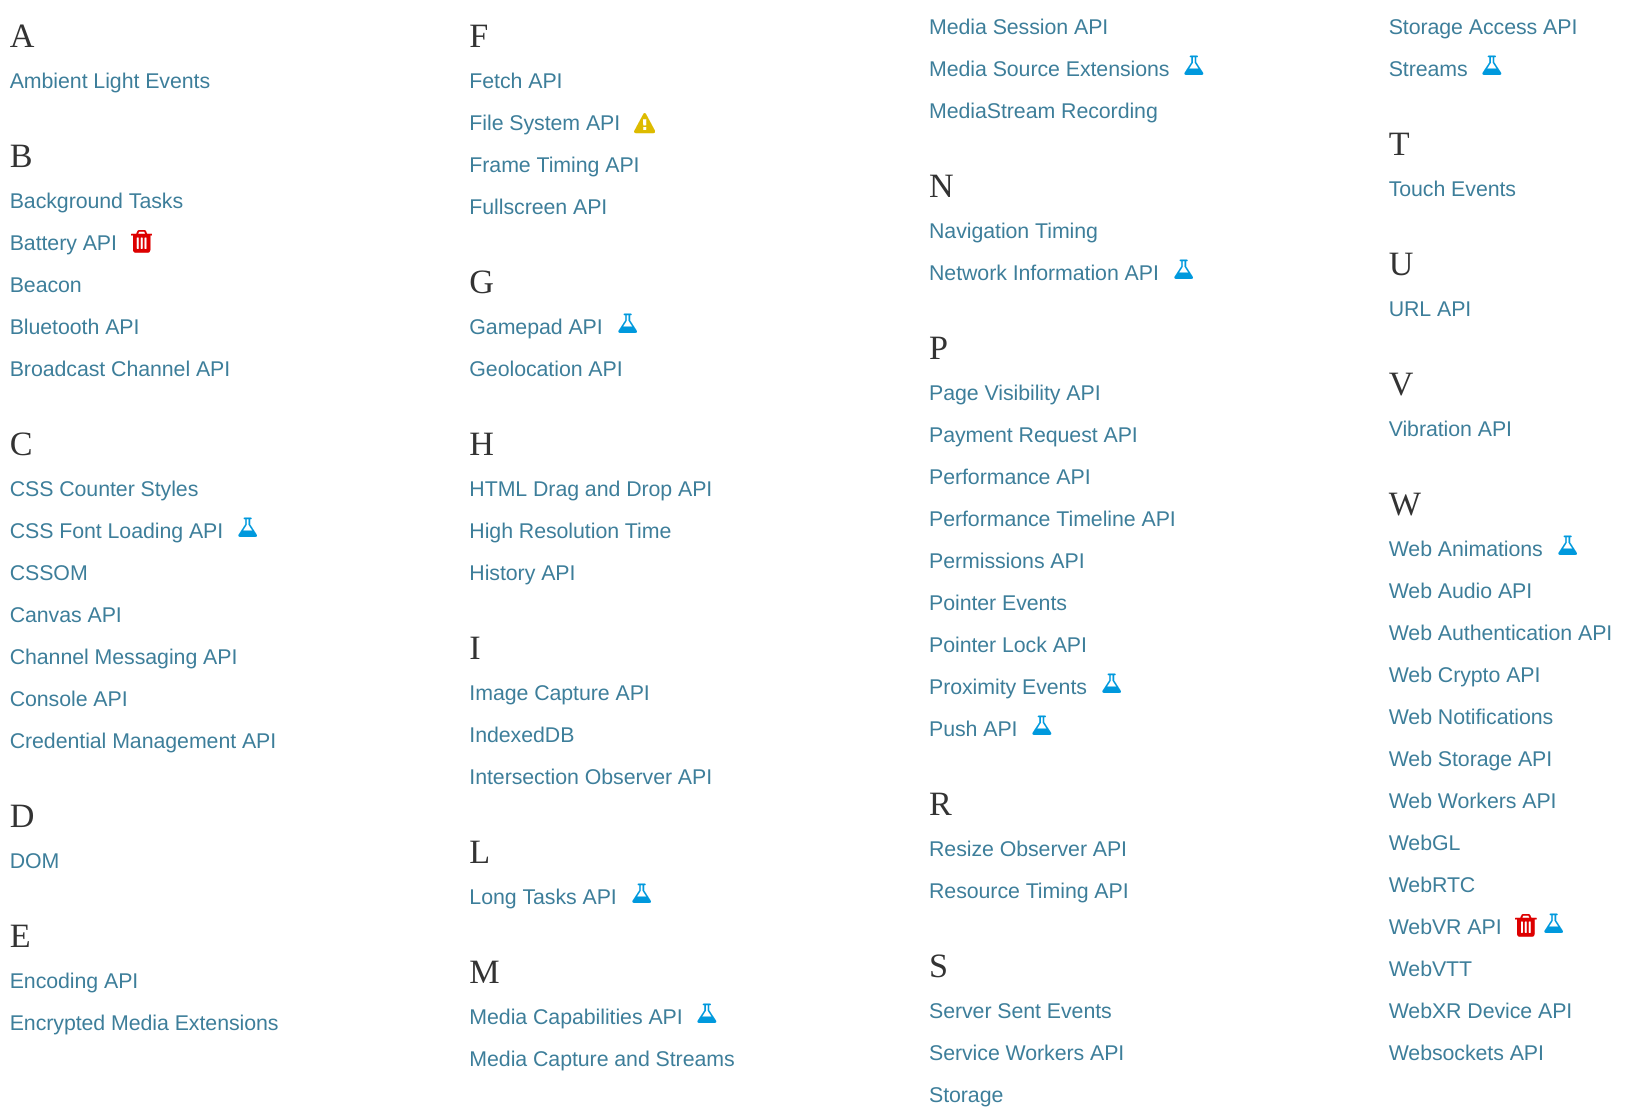
\includegraphics[width=1\textwidth]{Images/webapis.png}
	\caption{Lista de Web APIs}
	\label{fig:webAPIs}
\end{figure}


\subsection{\textit{Backend}}

En nuestro servidor \textit{backend} hemos optado por instalar XAMPP. Consiste en un paquete de herramientas para combinar las principales tecnologías que se utilizan en un servidor web. Hemos elegido este paquete de \textit{software} debido a la facilidades que brinda tanto para instalar como para usarse con el sistema operativo Microsoft Windows. Los componentes que hemos utilizado en XAMPP son los siguientes: \par

\subsubsection{Apache}

Es el servidor web más popular. Cuenta con una perfecta integración con los lenguajes que utilizamos, es decir PHP y JavaScript. \par 

Se trata de un servidor con el que ya habíamos trabajado anteriormente así que tomamos la decisión de utilizarlo para poder comenzar el desarrollo de nuestra aplicación rápidamente. También consideramos otras opciones que finalmente descartamos. Esto lo explicaremos en la sección~\ref{subsec:rejected}. \par 

\subsubsection{MaríaDB}

Se trata de un sencillo sistema gestor de base de datos relacionales. Es una bifurcación del proyecto MySQL, que fue adquirido por Sun Microsystems en 2009. El proyecto de MariaDB trata de dar continuación al desarrollo abierto de dicha tecnología a través de su comunidad. \par 

En nuestro proyecto se usa para albergar la huella digital que recopilamos de los navegadores web que conectan con nuestra aplicación. Como en el punto anterior, también consideramos otro tipo de bases de datos que finalmente fueron descartadas. \par 

\subsubsection{PhpMyAdmin}

Es una interfaz web para administrar la base de datos. Está escrita en PHP y soporta bases de datos tanto MariaDB como MySQL. \par 

Está contenida dentro de la instalación de XAMPP. Nos resulta más cómo observar el contenido de nuestra base de datos de un vistazo a través de una interfaz web y por eso utilizamos esta herramienta y no un cliente CLI. \par 

\subsection{Otras tecnologías}

Además de las tecnologías que hemos usado relacionadas con los navegadores, mencionamos el resto de tecnologías que hemos incorporado a nuestro proyecto: \par 

\subsubsection{Google Charts}

Utilizamos la herramienta Google Charts\cite{GoogleCharts} para representar estadísticas sobre la información que hemos almacenado en nuestra base de datos. A través de gráficas de tartas mostramos porcentajes de los atributos más comunes. Este herramienta la importamos a través de código JavaScript. \par 

\subsubsection{Git}

Es un \texit{software} de control de versiones. Nos permite organizar nuestro flujo de trabajo y guardar un historial de cambios para saber el motivo y la persona que realizó las nuevas mejoras. Además nos hace más sencilla la coordinación entre todo el equipo en el desarrollo de software. \par 

El código lo alojamos en la plataforma Github. Elegimos Github porque la licencia de estudiante ofrece una serie de extras de forma gratuita. Uno de estos extras es la opción de utilizar repositorios privados, en los que estábamos interesados. Igualmente, cuenta con una aplicación de escritorio que nos facilita la revisión de código antes de perpretar cambios definitivos. \par 

\subsubsection{PhpStorm}

Se trata de un entorno de desarrollo integrado (IDE) desarrollado por la compañía Jetbrains. Este IDE nos sorprendió por la cantidad de ayudas que nos ofrece al trabajar con PHP, JavaScript, HTML y CSS. Soporta todos esos lenguajes y formatos, además de contar con opciones de autocompletado de código y detección de errores sintácticos. \par 

Este entorno comercial es de pago. Sin embargo, cuenta con una licencia de estudiante que permite su uso gratuito. \par 

\subsubsection{\LaTeX}
\LaTeX es un sistema para componer textos. Se suele utilizar en textos técnicos y de divulgación científica. Su característica principal es que permite escribir documentos centrándose en el contenido del mismo, sin tener que preocuparse por los detalles del formato. Otra ventaja que ofrece es que la salida que ofrece es invariable, por lo que no depende del dispositivo con el que estamos trabajando. \par 

Usamos \LaTeX para componer el documento de la memoria del proyecto. \par 

Trabajamos con esta tecnología desde la página Overleaf. Nos decantamos por esta opción porque nos permite prescindir de descargar \textit{software} adicional en nuestra máquina. Asimismo, cuenta con diversos compiladores online, por lo que no tenemos que preocuparnos de los conflictos con las dependencias de los paquetes. \par 

\subsection{Tecnologías consideradas y finalmente descartadas}
\label{subsec:rejected}
Antes de elegir estuvimos probando con diversas tecnologías que finalmente fuimos descartando hasta quedarnos con las que hemos mencionado en el apartado anterior. Realizamos aquí un pequeño resumen. \par 

\subsubsection{Django}
Django es un framework de desarrollo web. Una de las ventajas es que respeta el patrón de diseño Modelo-Vista-Controlador (MVC). Por otra parte, el lenguaje de programación Python es usado en todas las partes del framework y no todos los integrantes del equipo tenemos el dominio suficiente sobre él. Finalmente consideramos que acostumbrarnos al lenguaje iba a resultar complicado y lo descartamos al estar más familiarizados con PHP. \par 

\subsubsection{Node.js}
Es un entorno en tiempo de ejecución construido sobre JavaScript, normalmente utilizado en el lado del servidor web. La principal ventaja que veíamos era la futura integración que podíamos tener más adelante con el código que recopila la información de la huella digital de los navegadores. Otra virtud a tener en cuenta es que con muy pocas líneas de código podíamos tener un servidor web escuchando y listo para producción. En comparación con Django que te obligaba a crear todos los componentes necesarios para respetar el modelo MVC, esto era mucho más rápido y sencillo. La complicación que le vimos era entender a fondo el lenguaje JavaScript, ya que al comienzo del proyecto nos sentíamos mucho más cómodos trabajando con PHP y Apache en el lado del servidor que con JavaScript y Node. \par 

\subsubsection{Nginx}
Es un servidor web. En cuanto a las características pensamos que es muy similar a Apache, por lo que no veíamos en Nginx ventajas considerables. Además, Apache ya viene incluido en el pack de herramientas de XAMPP. \par 

\subsubsection{MongoDB}
Nos planteamos la posibilidad de utilizar una base de datos NOSQL como MongoDB. La ventaja que le veíamos era el poder añadir atributos a medida que nos los íbamos encontrando, ya que en un primer momento al estudiar la diversidad de navegadores y configuraciones de los mismos, pensamos que podíamos encontrarnos con datos no estructurados. \par 

Sin embargo, vimos que no nos hacía falta ya que podíamos diseñar un esquema fijo relacional con tablas SQL. Además, la cantidad a datos a almacenar no tiene nada que ver con el entorno Big Data y MariaDB se adaptaba mejor a nuestras necesidades. \par 

\section{Herramientas similares}

Existen diversas herramientas similares a la que hemos desarrollado en nuestro proyecto, ya que todas realizan métodos de \textit{browser fingerprinting}. Sin embargo, las técnicas realizadas y los objetivos de cada plataforma son muy dispares. Hemos reunido en esta lista ejemplos de utilidades web que realizan \textit{browser fingerprinting}. Aclaramos aquí que existen varias herramientas a disposición del público. No obstante, estas son las que consideramos más representativas. \par

\subsubsection{AmIUnique}

AmIUnique\cite{amiunique} es una plataforma que recopila información de los diversos navegadores que visitan la web. De esta forma, son capaces de proveer estadísticas de uso. \par 
Entre sus objetivos encontramos:
\begin{itemize}
	\item Indicar si nuestra huella digital es única y si podemos llegar a ser rastreables.
	\item Mostrar el contenido de los parámetros más utilizados en \textit{browser fingerprinting}. Para cada parámetro, nos indica el porcentaje de registros similares encontrados en su base de datos.
	\item Estadísticas de uso globales: La herramienta nos muestra gráficos y porcentajes de los navegadores y sistemas operativos.
	\item Estadísticas de uso para ayudar a los desarrolladores para ayudarles ofrecer una experiencia optimizada para cada plataforma.
\end{itemize}

Los desarrolladores de esta plataforma también han diseñado una extensión de navegador para alertarnos de cuando nuestra huella digital ha cambiado. \par 

\subsubsection{Panopticlick}

Se trata de un proyecto de investigación de la \textit{Electronic Frontier Foundation} (EFF). Está desarrollado a partir la biblioteca \textit{Fingerprint2}\cite{fingerprintjs2} e incorpora partes de \textit{BrowserSpy.dk}\cite{browserSpy} para la detección de fuentes. \par 

El objetivo es concienciar a los usuarios de que son susceptibles a ser perfilados a través de su navegación. Para proteger nuestra privacidad, \textit{Panopticlick}\cite{panopticlick} recomienda la instalación de una extensión para el navegador, llamada \textit{Privacy Badger}, la cual ha sido también desarrollada por la EFF. Está disponible para Google Chrome, Mozilla Firefox y Opera Browser. \par 

\subsubsection{BrowserSpy.dk}

Encontramos aquí otra página diferente que nos permite averiguar la información que el navegador revela sobre nuestro dispositivo. \par 

Cuenta con un panel a la izquierda donde se hallan los distintos elementos que \textit{BrowserSpy}\cite{browserSpy} es capaz de obtener de nosotros. Pinchando sobre cada uno de ellos obtenemos el valor que se utiliza para rastrear nuestra huella digital. \par 

\subsubsection{BrowserLeaks}

\textit{BrowserLeaks}\cite{browserLeaks} es un portal web muy similar al anterior. En su página principal nos explica detalladamente cuales son los atributos que utiliza para obtener la huella digital del navegador web. \par 

Esta herramienta también tiene su menú a la izquierda con las distintas opciones que podemos escoger. Al pinchar sobre cada una de ellas obtenemos el dato usado para perfilarnos. \par 

\subsubsection{Audio Context Fingerprint TestPage}

Este proyecto forma parte del \textit{Princeton Web Transparency and Accountability Project}, de la Universidad de Princeton\cite{audio_page}. \par 

Al contrario que las plataformas anteriores, las cuales realizaban una comprobación más o menos completa de casi todas las habilidades conocidas de \textit{browser fingerprinting}, esta se focaliza tan solo es dos aspectos concretos. \par 

El objetivo es obtener la huella digital del navegador web analizando los valores de audio y detección de fuentes. \par 

En cuanto al audio, analiza las propiedades \textit{AudioContext}, \textit{DynamicsCompressor} y \textit{OscillatorNode}. \par 

También es posible obtener información de las distintas fuentes instaladas en el cliente, información del lienzo y detección de las fuentes de \textit{Flash}. \par 

\subsubsection{DeviceInfo}

\textit{Device Info}\cite{deviceinfo} es una utilidad que nos permite comprobar la privacidad de nuestros ajustes en el navegador. \par

El diseño de la página es muy austero; pero, a pesar de ello, cumple perfectamente con su cometido. Posiblemente sea la página más completa de todas en cuanto a la diversidad de técnicas que realiza para obtener la información del usuario. \par

Por contrapartida, no proporciona consejos para aumentar la privacidad de nuestro navegador web. Asimismo, tampoco nos devuelve los datos en un contexto en relación con otros usuarios. \par

